\newpage
\section{Applicability of Diffusion approximation}
\label{chapter:measurements}

The Diffusion approximation theory and BSSRDF model of rendering SSS materials has some strong
limitations for the optical properties of the materials (absorption coefficient, scattering
coefficient, and phase function) to be rendered and even geometric shape of the bounding
objects.

The restrictions on high volumetric albedo, high scattering and isotropism of the media makes it
impossible to render a full range of real world scattering materials with diffusion approximation.
There are some studies about the applicability of the Diffusion approximation with the descriptions
of the concrete limitations of this approach from practical point of view on supported materials
\cite{Donner:2009:EBM}, \cite{Gkioulekas:2013:URP:2516971.2516972},
\cite{Zhao:2014:HSR:2601097.2601104}. But these bounds on material properties are usually described
only in general terms.

One more way to define limitations of Diffusion approximation is described in this
section by estimating the difference with reference Monte Carlo rendered images and utilizing the
the results of measured properties of real media available in the literature.

\subsection{Measured data sources}
Scattering coefficients can be acquired by measuring diffusion profiles from a real-world object by
analyzing scattering of a laser beam \cite{Jensen:2001:PMS:383259.383319}.

Acquisition of the optical properties of human skin is a wide and important topic as
itself. Structured light patterns, for example, were used to estimate scattering coefficients of
different types of skin in \cite{tariq_efficient_2006-1}.

Rendering of translucent liquids is a bad potential case for rendering by Diffusion approximation
\textit{a priori}. Nevertheless the study of \cite{Narasimhan:2006:ASP:1141911.1141986}, containing
a big variety of liquids measured by dilution, appeared to be a valuable source of data.

The most recent up to date and comprehensive set of measured results is available in the work by
\cite{Gkioulekas:2013:IVR:2508363.2508377}. The advanced inverse volume rendering framework used in
that study allowed to take into account multiple scattering events and measure solids that are not
possible to dilute.

Data from all of these sources was used to estimate applicability of the Diffusion approximation
along with the Monte Carlo simulated samples.

\subsection{Experimental setup}
Searchlight experiment is a ubiquitous setup used in a number of research papers for developing
and analysing algorithms of light transport simulation in participating media. It is described in
section \ref{section:searchlight} and used for curve fitting and algorithm analysis in previous
section of this chapter. Being a simple and predictable model, it is far from the complexity
practical applications in production computer graphics.

Another approach was chosen here to measure visual consistency between the images rendered with
Diffusion approximation and references. In this work we have conducted experiments, similar to the
error measurement method used in \cite{Zhao:2014:HSR:2601097.2601104}. We rendered a wide range of
images containing a single object, while changing it's optical properties within a reasonable range
of possible values taking into account the characteristic scale of the object.

In contrast to the above mentioned work, we used ($1/\sigma_s, 1/\sigma_a$) space, as only
isotropic materials are interesting in our case of study. The difference between reference image and
Diffusion approximation rendered image represents one point in this space. The final results are
shown at figure \ref{fig:material_props}.

To reveal the quantitative limitations of Diffusion approximation we used two relatively complex
geometric models under two lighting conditions: a single side area light and an image based light
with HDR photos.

The path traced reference image is always show at the left in the next sections.

To make a conclusion about the limitations of the Diffusion approximation we rendered the
materials with absorption and scattering distances within the range of : $1/\sigma_a \in
[1,1000]$ mm and $1/\sigma_s \in [0.01,50]$ mm. While the characteristic scale of the details of
both models is about 5-50 mm. The full length of the Buckle is 50 mm, the Dragon is 100 mm.

\begin{figure}[h]
    \centering
    \begin{subfigure}{0.48\textwidth}
        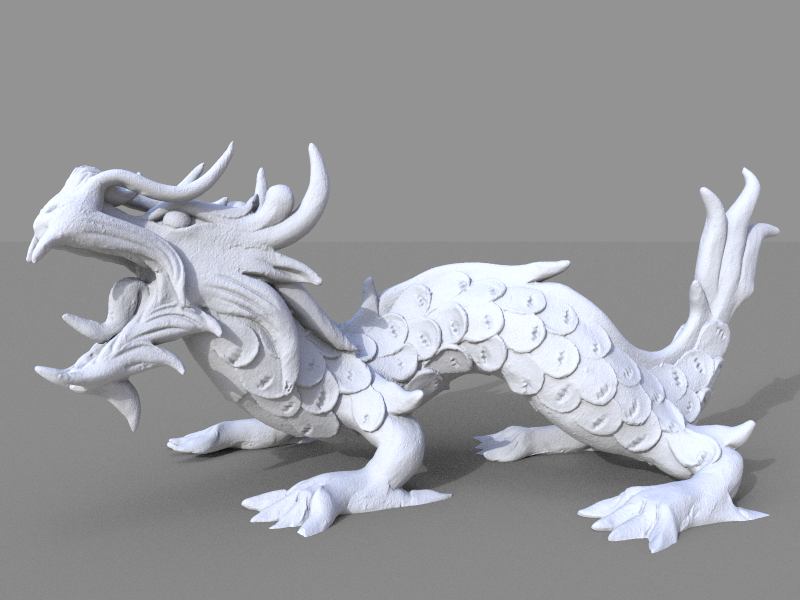
\includegraphics[width=\textwidth]{renders/xyzrgb_dragon_white}
        \caption{XYZRGB dragon. Scanned by Stanford Computer Graphics Laboratory}
    \end{subfigure}
    \begin{subfigure}{0.48\textwidth}
        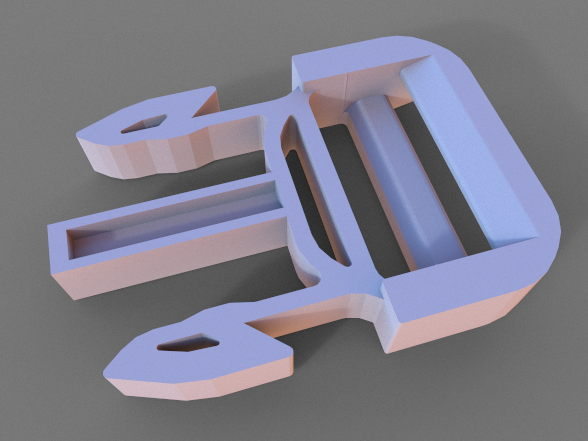
\includegraphics[width=\textwidth]{renders/buckle}
        \caption{Buckle. By Josip Vukovic from GrabCAD community digital library}
    \end{subfigure}
    \caption{3d models used for measurements}
    \label{fig:measurements_models}
\end{figure}

\subsection{Error measure}
\label{section:error_measure}
The \emph{Root Mean Square} (RMS) of the difference is a simple popular quantitative measure of the
error between two images. But it can not be used as a reasonable metric for comparison in our case,
because it depends too much on the absolute value of the image brightness difference. One example of
this is shown at figure \ref{fig:wrong_rms}. You can see the two pairs of images having similar RMS
error value $\approx 0.004$. But perceptual difference between two relatively dark images
\ref{fig:wrong_rms_dark} is considerably higher than one of brighter pair
\ref{fig:wrong_rms_bright}.
\begin{figure}[h]
    \centering
    \begin{subfigure}{0.4\textwidth}
        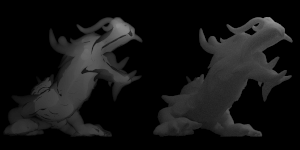
\includegraphics[width=\textwidth]{renders/matrix/rms000458}
        \caption{RMS=0.00458, high visual difference}
        \label{fig:wrong_rms_dark}
    \end{subfigure}
    \begin{subfigure}{0.4\textwidth}
        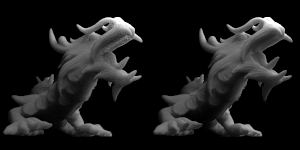
\includegraphics[width=\textwidth]{renders/matrix/rms000401}
        \caption{RMS=0.00401, low visual difference}
        \label{fig:wrong_rms_bright}
    \end{subfigure}
    \caption{Problem of RMS measure. Two pairs of images has close RMS error value. While perceived
    difference between the images of the left pair is much higher. Images are shown in 2x
    brightness}
    \label{fig:wrong_rms}
\end{figure}

That is why another metric was chosen. As a basis of calculation of the relative difference
between two images \emph{Normalized Cross-Correlation} was used:
\[
NCC = \frac{\sum_{x,y} (f(x,y)-\bar{f})(g(x,y)-\bar{g})}{N\sigma_f\sigma_g}
\]

where $f$ and $g$ are 2d functions $\bar{f}, \bar{g}$ are their mean values, $\sigma_f,\sigma_g$
respective standard deviations and $N$ is a number of pixels in case of images as a 2d functions.

General case of Cross-Correlation is often used for template matching in image processing. But in
our case it helps to measure the difference between two functions $f$ and $g$ regardless of their
mean value. Thus, it allows us to compute the error measure between various pairs of images
independent of their absolute average brightness. For the purpose of better representation and
visualization of the results, we re-parametrized the NCC value in the following way:
\[
C = \frac{\bar{f}}{\bar{g}}\frac{NCC^2-0.8}{0.2}
\]

It helps to represent the images with correlation only higher than 0.8 within the range [0,1].
The reason for this is that pairs with the NCC value lower than 0.8 are appeared to be unacceptable
visually wrong.
The factor $\bar{f}/\bar{g}$ is the ratio between average image brightness. It accounts for
relative difference of the Diffusion approximation image with the reference, not the absolute
difference, like in RMS case.

While using this metric, the images which appear very similar to their reference are represented by
C-value close to 1. And relatively wrong rendered images are having zero or near zero C-values
fig.\ref{fig:both_set}.

\subsection{Results}
\label{section:measurements_results}
In this section we present the generalized results of measurements described in two previous
sections.

\begin{figure}[h]
    \centering
    \begin{subfigure}{0.48\textwidth}
        
\includegraphics[width=\textwidth]{{{renders/matrix/area_buckle_da_100.0000_ds_0.0500}}}
        \caption{Buckle, area light. $1/\sigma_a=1000mm, 1/\sigma_s=0.5mm, C=0.745$}
    \end{subfigure}
    \quad
    \begin{subfigure}{0.48\textwidth}
        
\includegraphics[width=\textwidth]{{{renders/matrix/env_buckle_da_0.2000_ds_0.1000}}}
        \caption{Buckle, IBL. $1/\sigma_a=2mm, 1/\sigma_s=1mm, C=0.009$}
    \end{subfigure}
    \newline
    \begin{subfigure}{0.48\textwidth}
        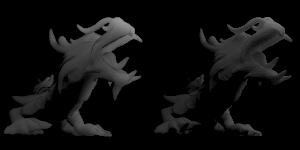
\includegraphics[width=\textwidth]{{{renders/matrix/area_dragon_da_1.0000_ds_0.2000}}}
        \caption{Dragon, area light. $1/\sigma_a=10mm, 1/\sigma_s=2mm, C=0.104$}
    \end{subfigure}
    \quad
    \begin{subfigure}{0.48\textwidth}
        
\includegraphics[width=\textwidth]{{{renders/matrix/env_dragon_da_30.0000_ds_0.0500}}}
        \caption{Dragon, IBL. $1/\sigma_a=300mm, 1/\sigma_s=5mm, C=0.793$}
    \end{subfigure}
    \caption{Two geometric shapes under two light setups. Left images of each pair is rendered using
    path tracing, right with Diffusion approximation. Examples of good and bad correlation using
    C-value metric from section
    \ref{section:error_measure}}
    \label{fig:both_set}
\end{figure}

\begin{figure}
    \includegraphics[width=\textwidth]{plots/matrix}
    \caption{Properties analysis draft}
    \label{fig:material_props}
\end{figure}